\chapter{Methodology}

\section{The Mediation Tool}
In order to address potential misuse of \gls{llm}-tools, we wanted to develop an interactive mediation tool aimed at teaching users of the inner workings of \gls{llms}. The intention was that by providing users with a viable mental model of how \gls{llms} work, they would be better equipped to use them in a responsible manner. We wanted to create an interactive tool that would engage users in a way that would be effective in showing them how the different components and aspects of \gls{llms} work together to produce the output they do. At the same time, the tool should be accessible to a wide range of users, not relying on prevoius technical or theoretical knowledge in \gls{cs} or \gls{ai}.

The intention was that participants in the study would use the tool to learn about \gls{llms} in their own time and at their own pace, without the need for instruction or guidance from us. Thus, it needed to be intuitive and engaging enough to encourage users to explore and learn on their own, keeping them inside the zone of proximal flow\ \cite{basawapatna_zones_2013}. We settled on a web-based tool containing a ``build your own \gls{llm}''-type experience, where users would be able to themselves choose and configure different components of a \gls{llm} and see how their choices would affect the output of the model. The technical implementation of the tool was done as a part of the Informatics Project II course at \gls{uib}, independent of this study, with David Grellscheid as supervisor. 

\subsection{Features}
\subsubsection*{The Dynamic Model}
The tool consists of various ways to interact with a very simple representation of a \gls{llm}. This model is modular, letting the users themselves choose which components and features they want to add to their model configuration. The model itself is a simple mapping between a token or sequence of tokens and the probability distribution of the next token. There are different versions of this mapping, depending on which features the user has selected in their configuration. There are 3 different tokenizers, 3 different context window sizes and a free choice of up to 2 out of 9 different books from Project Gutenberg\ \cite{gutenberg}. The model also contains a switch for whether the model should be deterministic by selecting the most probable token as the output, or non-deterministic by sampling from the probability distribution.

\subsubsection*{Build Your Own \gls{llm}}
The core feature of the tool is the ``Build Your Own \gls{llm}''-experience. In this view, users will be able to interact with a \gls{gui} containing a prompt-bar and a skill-tree of different components and configurations that they can choose to add to their model configuration. The prompt-bar will allow users to input prompts and then see the output of their model configuration in real-time, showing them the prediction for the next token as ghost text. The skill-tree displays all selected features in the current configuration, as well as all available features that can be added to the configuration. The features are organized in a tree structure, in order to demonstrate the dependencies between different components and configurations. For example, you cannot select the 3-context-window feature without first selecting the 2-context-window feature. 

\begin{figure}
    \centering
    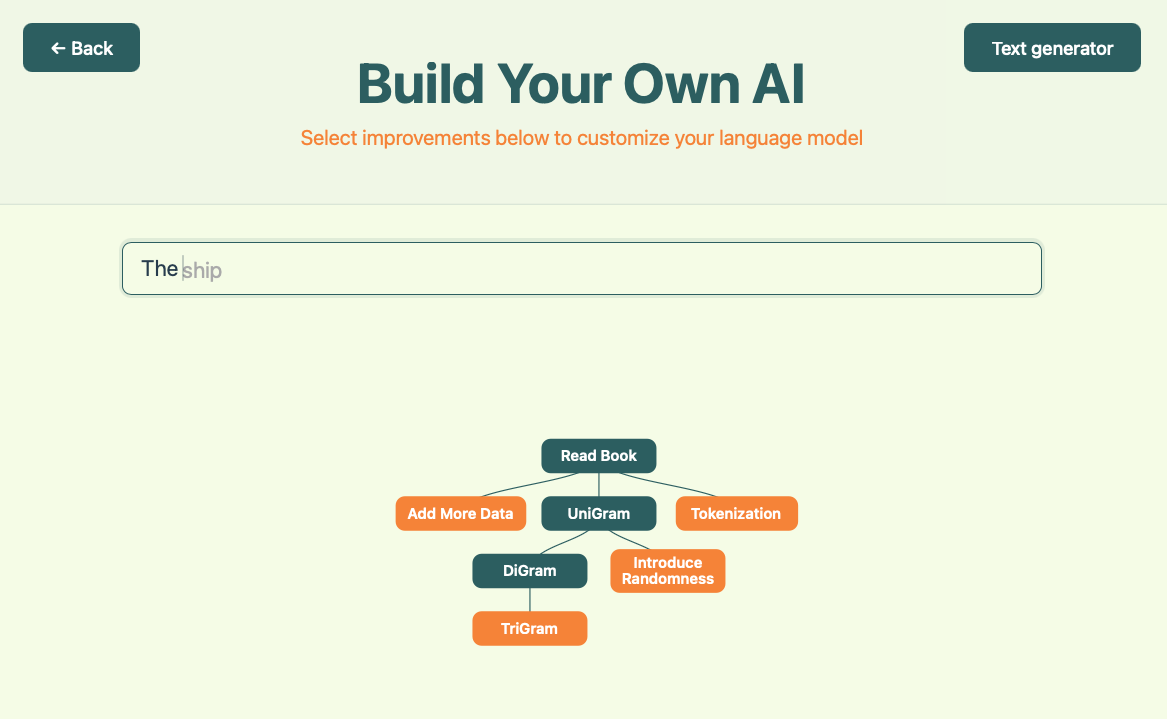
\includegraphics[scale=0.3]{figures/builder_page.png}
    \caption{The ``Build Your Own LLM''-view of the mediation tool.}
    \label{BuilderPageFigure}
\end{figure}

\subsubsection*{Text Generator}
At any point in the ``Build Your Own \gls{llm}''-experience, users can explore their current configuration in a text generation context. By clicking the ``Text Generator''-button, users are taken to a different view containing a larger text input field and a button saying ``Generate Text''. Here, users can input longer prompts and at any point click the ``Generate Text''-button to have their current model configuration continously generate the next token in the text, like a normal \gls{llm} would. This also demonstartes to the users that the same underlying process can be used for multiple purposes, and that the different features they have selected in the skill-tree work together to produce the output of the model.

\begin{figure}
    \centering
    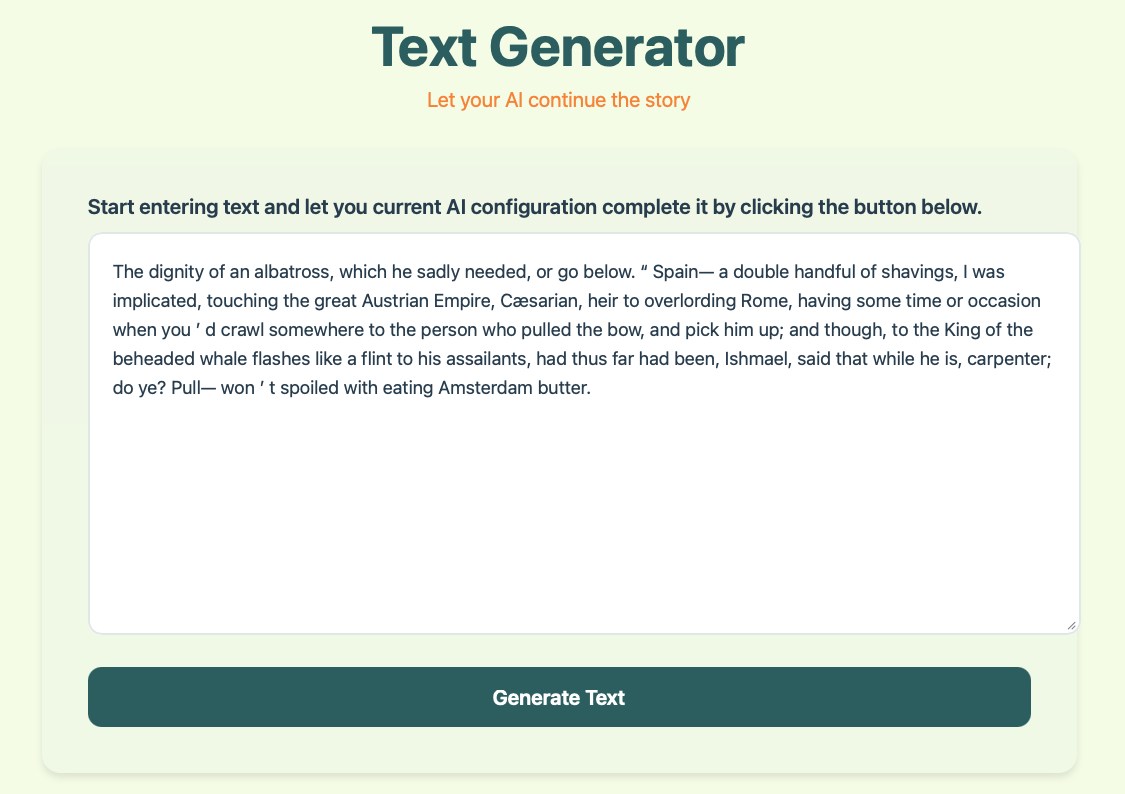
\includegraphics[scale=0.3]{figures/text_generator_page.png}
    \caption{The ``Text Generator''-view of the mediation tool.}
    \label{TextGeneratorPageFigure}
\end{figure}

\subsubsection*{Scrollytelling Chapters}
Connected to each feature in the skill-tree is a scrollytelling chapter that explains the feature in more detail. Scrollytelling is a form of interactive storytelling where the content visible on the screen changes as the user scrolls down the page. This is utilized in the mediation tool to provide users with a more engaging and interactive way to learn about the different features and components of \gls{llms}. Each chapter consists of a collection of textboxes, to each of which have a coresponding visual animation that is triggered when the textbox is scrolled into view. The animations are designed to visually demonstrate the concepts explained in the textboxes, providing users with a more intuitive understanding of how the different features and components of \gls{llms} work together to produce the output they do.

\begin{figure}
    \centering
    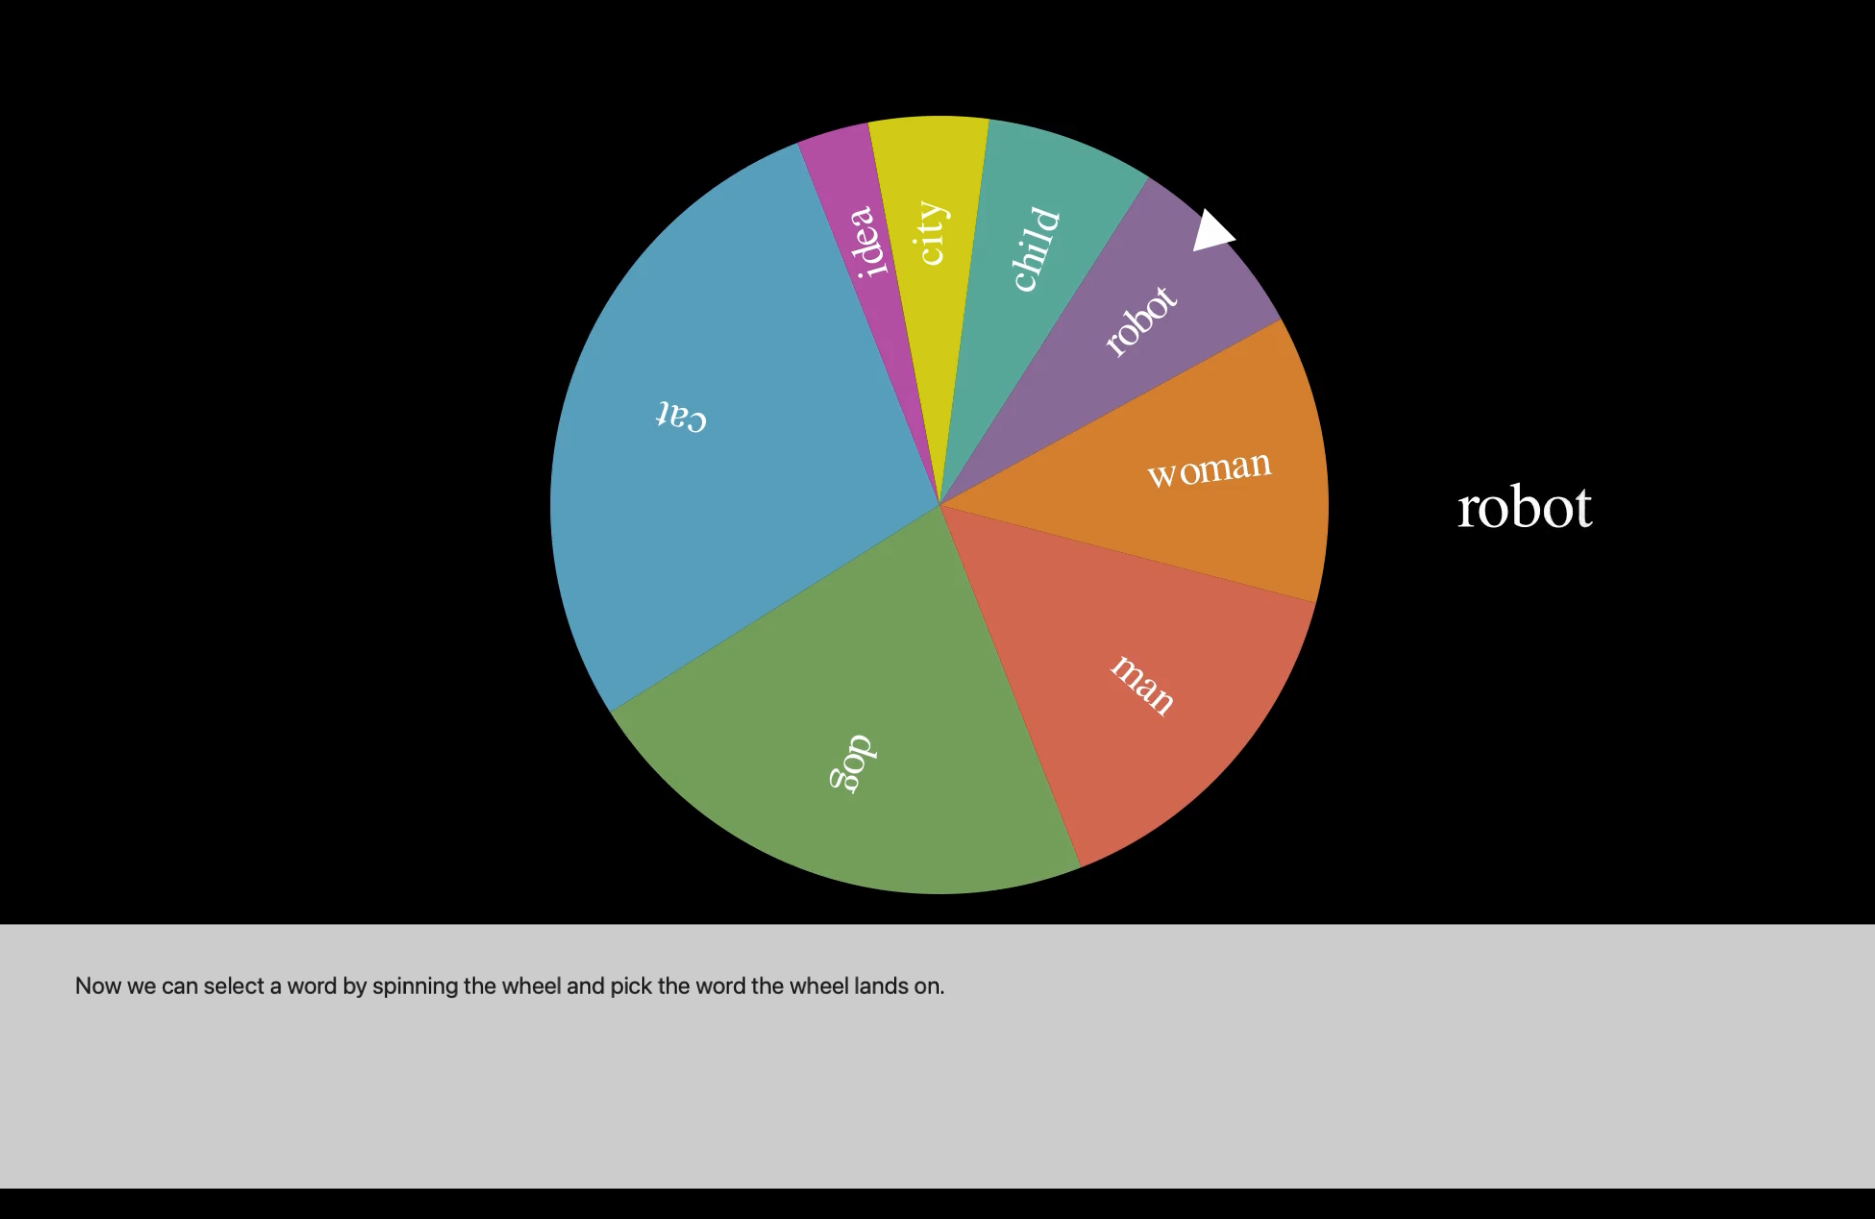
\includegraphics[scale=0.2]{figures/scrollytelling_page.png}
    \caption{The scrollytelling chapter connected to the weighted random sampling feature.}
    \label{ScrollytellingPageFigure}
\end{figure}

\subsubsection*{Chapter Overview}
Users can at any point access each of the individual scrollytelling chapters through a chapter overview page. This page contains a list of all the features available in the tool, organized by category. Each feature has a short description, and by clicking on the feature, users are taken to the corresponding scrollytelling chapter where they can learn more about the feature and how it works.

\subsubsection*{External Resources}
At the bottom of the chapter overview page, there is a section containing a list of external resources for users who want to learn more about \gls{llms} and how they work. This includes online courses, educational videos, articles and blog posts on relevant topics\ \cite{bergstrom_west_bullshit_machines,cho_transformer_explainer_2024,google_pair_explorables,perret_not_writing_chatgpt_2024,sanderson_llm_explained_video,savetheai_website,stollnitz_gpt_works_2023}.

\subsection{\gls{llm} Representation}
The mediation tool does not actually contain a real transformer-based \gls{llm} under the hood, but rather a simple representation of one. Each branch of the skill tree corresponds to a different feature or component of \gls{llms}. Most of the topics contain multiple chapters building on each other, to keep users in the zone of proximal flow\ \cite{basawapatna_zones_2013}.

\begin{figure}[h]
\centering
\begin{tikzpicture}[
  every node/.style={font=\small},
  edge style/.style={->, >=latex, thick},
  base/.style   ={circle, thick, minimum size=4em, inner sep=3pt, align=center, font=\scriptsize},
  train/.style  ={base, draw=blue!70,         fill=blue!20},
  context/.style={base, draw=green!60!black,  fill=green!20},
  temp/.style   ={base, draw=red!70,          fill=red!20},
  tok/.style    ={base, draw=orange!80!black, fill=orange!20},
  legendbox/.style={rectangle, draw, thick, minimum size=1em, inner sep=0pt},
]

% ── Nodes ──────────────────────────────────────────────────────────
\node[train]   (rb)  at (0,    0)  {Read\\Book};
\node[train]   (ra)  at (-2,  -3)  {Read\\Another};
\node[train]   (sc)  at (-2,  -6)  {Select\\Corpus};
\node[context] (og)  at (2,   -3)  {Unigram};
\node[context] (tg)  at (1,   -6)  {Digram};
\node[context] (trg) at (1,   -9)  {Trigram};
\node[temp]    (wr)  at (3,   -6)  {Weighted\\Random};
\node[tok]     (tok) at (6,   -3)  {Tokenization};
\node[tok]     (nl)  at (6,   -6)  {Language\\Awareness};

% ── Edges ──────────────────────────────────────────────────────────
\draw[edge style] (rb)  -- (ra);
\draw[edge style] (ra)  -- (sc);
\draw[edge style] (rb)  -- (og);
\draw[edge style] (og)  -- (tg);
\draw[edge style] (tg)  -- (trg);
\draw[edge style] (og)  -- (wr);
\draw[edge style] (rb)  -- (tok);
\draw[edge style] (tok) -- (nl);

% ── Legend ─────────────────────────────────────────────────────────
\node[legendbox, fill=blue!20,   draw=blue!70]         (l1) at (9, -1)   {};
\node[right=4pt of l1, font=\scriptsize] {Training Data};

\node[legendbox, fill=green!20,  draw=green!60!black]  (l2) at (9, -1.6) {};
\node[right=4pt of l2, font=\scriptsize] {Context};

\node[legendbox, fill=red!20,    draw=red!70]           (l3) at (9, -2.2) {};
\node[right=4pt of l3, font=\scriptsize] {Temperature};

\node[legendbox, fill=orange!20, draw=orange!80!black]  (l4) at (9, -2.8) {};
\node[right=4pt of l4, font=\scriptsize] {Tokenization};

\node[draw, rounded corners, inner sep=6pt,
      fit=(l1)(l2)(l3)(l4),
      label={[font=\small\bfseries]above:Legend}] {};

\end{tikzpicture}
\caption{Selection tree with grouped LLM features}
\label{fig:selection-tree}
\end{figure}